% Options for packages loaded elsewhere
% Options for packages loaded elsewhere
\PassOptionsToPackage{unicode}{hyperref}
\PassOptionsToPackage{hyphens}{url}
\PassOptionsToPackage{dvipsnames,svgnames,x11names}{xcolor}
%
\documentclass[
  11pt,
]{article}
\usepackage{xcolor}
\usepackage[top=0.4in,bottom=0.45in,left=0.65in,right=0.65in,includehead,headheight=52pt,headsep=7pt,includefoot,footskip=24pt]{geometry}
\usepackage{amsmath,amssymb}
\setcounter{secnumdepth}{-\maxdimen} % remove section numbering
\usepackage{iftex}
\ifPDFTeX
  \usepackage[T1]{fontenc}
  \usepackage[utf8]{inputenc}
  \usepackage{textcomp} % provide euro and other symbols
\else % if luatex or xetex
  \usepackage{unicode-math} % this also loads fontspec
  \defaultfontfeatures{Scale=MatchLowercase}
  \defaultfontfeatures[\rmfamily]{Ligatures=TeX,Scale=1}
\fi
\usepackage{lmodern}
\ifPDFTeX\else
  % xetex/luatex font selection
\fi
% Use upquote if available, for straight quotes in verbatim environments
\IfFileExists{upquote.sty}{\usepackage{upquote}}{}
\IfFileExists{microtype.sty}{% use microtype if available
  \usepackage[]{microtype}
  \UseMicrotypeSet[protrusion]{basicmath} % disable protrusion for tt fonts
}{}
\makeatletter
\@ifundefined{KOMAClassName}{% if non-KOMA class
  \IfFileExists{parskip.sty}{%
    \usepackage{parskip}
  }{% else
    \setlength{\parindent}{0pt}
    \setlength{\parskip}{6pt plus 2pt minus 1pt}}
}{% if KOMA class
  \KOMAoptions{parskip=half}}
\makeatother
% Make \paragraph and \subparagraph free-standing
\makeatletter
\ifx\paragraph\undefined\else
  \let\oldparagraph\paragraph
  \renewcommand{\paragraph}{
    \@ifstar
      \xxxParagraphStar
      \xxxParagraphNoStar
  }
  \newcommand{\xxxParagraphStar}[1]{\oldparagraph*{#1}\mbox{}}
  \newcommand{\xxxParagraphNoStar}[1]{\oldparagraph{#1}\mbox{}}
\fi
\ifx\subparagraph\undefined\else
  \let\oldsubparagraph\subparagraph
  \renewcommand{\subparagraph}{
    \@ifstar
      \xxxSubParagraphStar
      \xxxSubParagraphNoStar
  }
  \newcommand{\xxxSubParagraphStar}[1]{\oldsubparagraph*{#1}\mbox{}}
  \newcommand{\xxxSubParagraphNoStar}[1]{\oldsubparagraph{#1}\mbox{}}
\fi
\makeatother


\usepackage{longtable,booktabs,array}
\usepackage{calc} % for calculating minipage widths
% Correct order of tables after \paragraph or \subparagraph
\usepackage{etoolbox}
\makeatletter
\patchcmd\longtable{\par}{\if@noskipsec\mbox{}\fi\par}{}{}
\makeatother
% Allow footnotes in longtable head/foot
\IfFileExists{footnotehyper.sty}{\usepackage{footnotehyper}}{\usepackage{footnote}}
\makesavenoteenv{longtable}
\usepackage{graphicx}
\makeatletter
\newsavebox\pandoc@box
\newcommand*\pandocbounded[1]{% scales image to fit in text height/width
  \sbox\pandoc@box{#1}%
  \Gscale@div\@tempa{\textheight}{\dimexpr\ht\pandoc@box+\dp\pandoc@box\relax}%
  \Gscale@div\@tempb{\linewidth}{\wd\pandoc@box}%
  \ifdim\@tempb\p@<\@tempa\p@\let\@tempa\@tempb\fi% select the smaller of both
  \ifdim\@tempa\p@<\p@\scalebox{\@tempa}{\usebox\pandoc@box}%
  \else\usebox{\pandoc@box}%
  \fi%
}
% Set default figure placement to htbp
\def\fps@figure{htbp}
\makeatother





\setlength{\emergencystretch}{3em} % prevent overfull lines

\providecommand{\tightlist}{%
  \setlength{\itemsep}{0pt}\setlength{\parskip}{0pt}}



 


% =====================================================================
%  _style.tex  ·  Design system for EIL research highlights (v4 layout)
%  Edit here to restyle ALL research highlights. Included via the .qmd YAML.
%  Matches the canonical single-column v4 template; the masthead and footer
%  are set per-document via fancyhdr in each .qmd's include-in-header.
% =====================================================================

% ---- Colours (exact hex) --------------------------------------------
\definecolor{ink}{HTML}{1D2620}        % headings, title, section heads, rule
\definecolor{body}{HTML}{33352C}       % main body paragraphs
\definecolor{accentred}{HTML}{641111}  % RESEARCH HIGHLIGHT label, links, fig title
\definecolor{boxred}{HTML}{8C2826}     % Bottom Line box fill
\definecolor{boxtext}{HTML}{EEF1EA}    % Bottom Line body text (off-white)
\definecolor{muted}{HTML}{50534A}      % figure source line
\definecolor{cite}{HTML}{6E6D61}       % citation line
\definecolor{faint}{HTML}{9A978A}      % footer
\definecolor{warmrule}{HTML}{D8D2C2}   % thin warm-grey dividers
\definecolor{paper}{HTML}{FAF8F1}      % warm page background

% \pagecolor{paper}                    % uncomment for warm off-white background

% ---- Fonts (Source Sans 3 / Source Serif 4) -------------------------
\usepackage[T1]{fontenc}
\usepackage[default]{sourcesanspro}
\usepackage{sourceserifpro}
\renewcommand{\familydefault}{\sfdefault}

% ---- Page -----------------------------------------------------------
\pagestyle{empty}
\setlength{\parindent}{0pt}
\setlength{\parskip}{2pt}
% Default body size/colour. The v4 .qmd overrides this to 10.5/13.5pt.
\AtBeginDocument{\color{body}\fontsize{9.4pt}{13.6pt}\selectfont}

% ---- Packages -------------------------------------------------------
\usepackage{microtype}
\usepackage{soul}
\setul{2pt}{.5pt}
\usepackage{tcolorbox}
\tcbuselibrary{skins}
\usepackage[colorlinks=true, urlcolor=accentred, linkcolor=accentred, pdfborder={0 0 0}]{hyperref}

% =====================================================================
%  MACROS
% =====================================================================

% --- Title + citation (citation has a thin warm divider beneath) ------
\newcommand{\brieftitle}[1]{%
  {\color{ink}\fontsize{18pt}{19.5pt}\selectfont\bfseries\textls[-12]{#1}\par}\vspace{3pt}}
\newcommand{\briefcitation}[1]{%
  {\color{cite}\fontsize{9.4pt}{12pt}\selectfont #1\par}\vspace{3pt}%
  \noindent\textcolor{warmrule}{\rule{\linewidth}{0.7pt}}}

% --- Section heads (uppercase, ink) ----------------------------------
\newcommand{\sectionhead}[1]{%
  \vspace{2pt}{\color{ink}\bfseries\fontsize{9.75pt}{12pt}\selectfont
  \textls[20]{\MakeUppercase{#1}}\par}\vspace{1pt}}

% --- Sub-heads (small uppercase) — Takeaway subheads -----------------
% The v4 .qmd overrides this to the brand maroon via \renewcommand.
\newcommand{\subhead}[1]{%
  {\color{ink}\bfseries\fontsize{8.25pt}{10pt}\selectfont
  \textls[50]{\MakeUppercase{#1}}\par}\vspace{2pt}}

% --- Figure title + source line --------------------------------------
\newcommand{\figtitle}[2]{%
  {\bfseries\color{accentred}\fontsize{7.1pt}{9pt}\selectfont\textls[40]{\MakeUppercase{#1}}}\par%
  {\color{muted}\fontsize{7.1pt}{9pt}\selectfont #2}\par\vspace{4pt}}

% =====================================================================
%  COLOURED BOXES
% =====================================================================

% --- Bottom Line box (border-radius 6px -> arc=4pt) ------------------
\newtcolorbox{bottomline}{%
  enhanced, arc=4pt, outer arc=4pt, boxrule=0pt,
  colback=boxred, coltext=boxtext,
  left=7pt, right=7pt, top=7pt, bottom=7pt,
  before upper={\fontsize{9.4pt}{13.6pt}\selectfont}}

% --- Info box (contact + full citation; centered, thin faint border) --
% Superseded by the moreinfo environment below; kept so older highlights
% still compile. Faint text at footer size. Wrap any link as
% \href{url}{\color{faint}\underline{text}} so it inherits the faint
% colour instead of the global accent link colour.
\newtcolorbox{infobox}{%
  enhanced, width=0.9\linewidth, center, arc=4pt, outer arc=4pt,
  boxrule=0.5pt, colframe=faint, colback=white, coltext=faint,
  left=9pt, right=9pt, top=7pt, bottom=7pt,
  before upper={\fontsize{7.4pt}{9.5pt}\selectfont}}

% =====================================================================
%  CLOSING BLOCK
% =====================================================================

% --- For more information (full width; rule above, no box) ------------
% Citation, author affiliations + contact, then the EIL boilerplate —
% one paragraph each. Wrap any link as
% \href{url}{\color{cite}\underline{text}} so it inherits the block's
% grey instead of the global accent link colour.
\newenvironment{moreinfo}{%
  \par\vspace{12pt}%
  \noindent\textcolor{warmrule}{\rule{\linewidth}{0.7pt}}\par
  \vspace{7pt}%
  {\color{ink}\bfseries\fontsize{8.25pt}{10pt}\selectfont
   \textls[50]{\MakeUppercase{For more information}}\par}\vspace{4pt}%
  \color{cite}\fontsize{8.4pt}{11.5pt}\selectfont
  \setlength{\parskip}{5pt}%
}{\par}
% --- Running masthead + footer (logo, label, rule, page number) ---
\usepackage{fancyhdr}
\renewcommand{\headrulewidth}{0pt}
\renewcommand{\footrulewidth}{0pt}
\fancypagestyle{brief}{%
  \fancyhf{}%
  \fancyhead[L]{%
    \begin{minipage}[c]{0.62\textwidth}\raggedright\color{ink}
\includegraphics[height=0.45in]{../../../formats/logos/eil-logo-maroon.png}\end{minipage}\hfill%
    \begin{minipage}[c]{0.36\textwidth}\raggedleft\fontsize{8.25pt}{10pt}\selectfont\bfseries\color{accentred}\textls[200]{\MakeUppercase{Research Highlight}}\end{minipage}%
    \par\vspace{2pt}%
    \noindent\textcolor{ink}{\rule{\textwidth}{2.2pt}}%
  }%
  \fancyfoot[C]{%
    \color{warmrule}\rule{\textwidth}{0.7pt}\par\vspace{3pt}%
    \hbox to\textwidth{%
      \color{faint}\fontsize{7.4pt}{9pt}\selectfont
      For full paper:\hspace{0.4em}\href{https://doi.org/10.1162/rest_a_01395}{\color{faint}\underline{\textls[40]{doi.org/10.1162/rest\_a\_01395}}}%
      \hfill
      Page \thepage%
    }%
  }%
}
\pagestyle{brief}
\renewcommand{\subhead}[1]{%
  {\color{accentred}\bfseries\fontsize{8.25pt}{10pt}\selectfont
  \textls[50]{\MakeUppercase{#1}}\par}\vspace{2pt}}
\makeatletter
\@ifpackageloaded{caption}{}{\usepackage{caption}}
\AtBeginDocument{%
\ifdefined\contentsname
  \renewcommand*\contentsname{Table of contents}
\else
  \newcommand\contentsname{Table of contents}
\fi
\ifdefined\listfigurename
  \renewcommand*\listfigurename{List of Figures}
\else
  \newcommand\listfigurename{List of Figures}
\fi
\ifdefined\listtablename
  \renewcommand*\listtablename{List of Tables}
\else
  \newcommand\listtablename{List of Tables}
\fi
\ifdefined\figurename
  \renewcommand*\figurename{Figure}
\else
  \newcommand\figurename{Figure}
\fi
\ifdefined\tablename
  \renewcommand*\tablename{Table}
\else
  \newcommand\tablename{Table}
\fi
}
\@ifpackageloaded{float}{}{\usepackage{float}}
\floatstyle{ruled}
\@ifundefined{c@chapter}{\newfloat{codelisting}{h}{lop}}{\newfloat{codelisting}{h}{lop}[chapter]}
\floatname{codelisting}{Listing}
\newcommand*\listoflistings{\listof{codelisting}{List of Listings}}
\makeatother
\makeatletter
\makeatother
\makeatletter
\@ifpackageloaded{caption}{}{\usepackage{caption}}
\@ifpackageloaded{subcaption}{}{\usepackage{subcaption}}
\makeatother
\usepackage{bookmark}
\IfFileExists{xurl.sty}{\usepackage{xurl}}{} % add URL line breaks if available
\urlstyle{same}
\hypersetup{
  colorlinks=true,
  linkcolor={blue},
  filecolor={Maroon},
  citecolor={Blue},
  urlcolor={Blue},
  pdfcreator={LaTeX via pandoc}}


\author{}
\date{}
\begin{document}


% ---------------------------------------------------------------------
% TITLE + CITATION
% ---------------------------------------------------------------------
\brieftitle{Hot Days Turn Deadlier Where Guns Are Easy to Carry}

% OUTLINE — citation line:
%   - exact paper title in straight quotes, both authors, journal + year
%   - RESOLVED: Review of Economics and Statistics, 2026, 108(1): 30-43
\briefcitation{Lessons from ``Access to Guns in the Heat of the Moment: More Restrictive Gun Laws Mitigate the Effect of Temperature on Violence'' by Jonathan Colmer \& Jennifer L. Doleac in \textit{The Review of Economics and Statistics}, 2026.}

\vspace{-2pt}
\fontsize{10.5pt}{13.5pt}\selectfont

% ---------------------------------------------------------------------
% BOTTOM LINE (~40-50 words, one bold sentence + 1-2 more)
% ---------------------------------------------------------------------
% OUTLINE:
%   - bold sentence: heat drives up homicides, but stricter concealed-
%     carry laws blunt most of that effect
%   - need to pick ONE headline comparison stat and use it consistently
%     everywhere in the doc (title, bottom line, found section):
%       option A: More-Prohibitive vs Less-Prohibitive baseline temp
%         coefficients from Table 2 Panel B/C, col (2): 0.000430 vs
%         0.000657 -> ~35% smaller heat effect under stricter laws
%       option B: DiT estimate itself, -0.000511, framed against the
%         paper's own baseline comparison (0.000641) -> a much larger
%         reduction (~80%), but mixes specifications -- riskier to cite
%         without the same caveats the paper gives
%       -> RECOMMEND option A for the highlight (cleaner apples-to-
%          apples, same specification, easy for a lay reader to verify
%          against the figure); flag this choice to Josie before
%          drafting prose
%   - second sentence: why it matters — gun violence is already the
%     leading cause of death for young Black Americans; climate change
%     means more hot days ahead
% Swapped the self-derived fraction for the paper's own directly-stated
% figure (299 additional homicides/year, for today's looser-law states
% specifically) -- see chat for why a derived percentage/fraction wasn't
% safe to present as paper-stated, and why this is annualized, not a
% single-hot-day figure.
\begin{bottomline}
{\fontsize{11pt}{15pt}\selectfont
\textbf{Hot days lead to more gun homicides, but stricter concealed-carry laws sharply cut that effect.} In today's looser-law states, a year of days running one degree hotter than normal is estimated to cause roughly 299 more homicides than those same states would see under stricter laws.
}
\end{bottomline}

\vspace{6pt}

% ---------------------------------------------------------------------
% BACKGROUND (~180 words, 2 paragraphs)
% ---------------------------------------------------------------------
\sectionhead{Background}

% OUTLINE — paragraph 1 (the two things we already know, per your framing):
%   - established fact #1: hotter days -> more violent crime (cite this
%     as settled science, not news -- prior lab/field studies: horn
%     honking, police firearms training, baseball beanballs, prison
%     violence w/o AC)
%   - established fact #2: not all states treat carrying a concealed
%     gun the same way -- define term in bold on first use, plain-
%     language spectrum (basically unrestricted -> permit required for
%     anyone who asks -> permit at official's discretion -> banned),
%     collapsed for the reader into "easier to carry" vs "harder to
%     carry"
%   - bridge to the open question: if heat makes people more prone to
%     violence, does whether a gun is close at hand change how that
%     plays out? end paragraph on this question
%
% OUTLINE — paragraph 2 (setting/data, plain language):
%   - data: daily police crime reports (NIBRS) covering ~5,900 police
%     jurisdictions, 1991-2016, matched day-by-day to local weather
%     records and to each state's concealed-carry rules that month
%   - why homicide as the outcome: most consistently/reliably reported
%     crime type, so it's not just a story about reporting differences
%   - close on setup for "what the study found": with this data they
%     can watch what happens to homicides on hot days, specifically in
%     places/times with stricter vs. looser carry laws
\noindent Gun violence is a large problem in the United States. Given the research that has established that high temperatures lead to increased aggression and violent behavior, this problem will only increase as temperatures rise due to climate change. Additionally, states differ significantly in their \textbf{concealed-carry laws} --- the rules governing who can carry a hidden handgun in public. Some states let nearly any adult carry one; others require a permit that officials can deny, or ban concealed carry altogether. Together, these two facts raise an important question: \textbf{if heat makes people more likely to become violent, does having a gun close at hand change the results of these confrontations?} If so, then stricter concealed-carry laws may protect against an increase in homicides as temperatures rise.

\noindent To answer this question, researchers matched 25 years of daily police crime reports (1991--2016) with local weather records and each state's concealed-carry laws, month by month. This allowed them to understand the temperature and laws in place at the time of every gun violence homicide.

\vspace{6pt}

\begin{center}
\begin{minipage}{0.82\linewidth}
\figtitle{How much hotter days raise homicides, depending on how strict a state's gun laws are}{Source: Colmer \& Doleac (2026).}
% NOTE: values in this figure are approximated from the published
% Figure 2 image, not sourced from a replication package (none found
% publicly) -- confirm with Colmer & Doleac before this goes public.
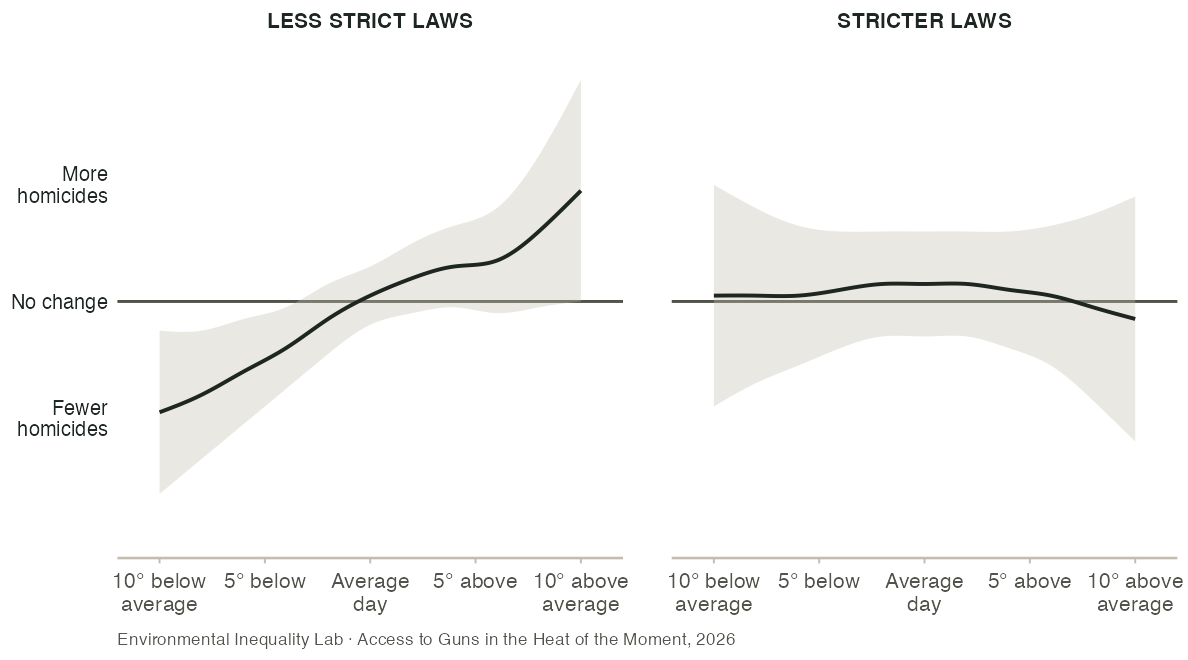
\includegraphics[width=\linewidth]{../data-viz/figures/fig1-temp-homicide-by-regime.png}
\par\vspace{3pt}
{\color{faint}\fontsize{7.1pt}{9.5pt}\selectfont \textit{Note:} Each panel shows the estimated relationship between daily temperature and homicides, after accounting for typical seasonal and local patterns. In states with less strict concealed-carry laws (left), hotter days correlate with more homicides. In states with stricter laws (right), the flatter line indicates that homicides do not increase with hotter weather. The shaded areas show the range of uncertainty around each estimate.\par}
\end{minipage}
\end{center}
% ---------------------------------------------------------------------
% WHAT THE STUDY FOUND (~300 words + figure, two-page budget)
% ---------------------------------------------------------------------
\newpage
\sectionhead{What the study was}

% ---------------------------------------------------------------------
% FIGURE — adapted Figure 2 (temperature-homicide relationship by
% policy regime), house style
% ---------------------------------------------------------------------
% OUTLINE — figure:
%   - source figure: paper's Figure 2, semi-parametric temperature-
%     homicide relationship, plotted separately for less-prohibitive
%     and more-prohibitive concealed-carry states
%   - figtitle (sentence-style, describes what's shown, not the method)
%   - build script: code/make-fig1-temp-homicide-by-regime.R
%     -> figures/fig1-temp-homicide-by-regime.png
%     (approximated from the published figure -- no replication package
%     found publicly; check with PIs before this goes public)
%   - note (plain language, how to read + what to conclude):
%     - less-strict-law states: line rises with temperature -- hotter
%       days bring more homicides
%     - stricter-law states: line stays flat -- hotter days aren't any
%       more dangerous

% OUTLINE — design narrative (walk the reader through the reasoning,
% per style guide's "storytelling" instruction -- don't name DiD/DiT):
%   - naive start: just compare hot days to cold days everywhere -> but
%     hot places and cold places differ in a thousand other ways
%     (poverty, policing, culture) that also affect violence
%   - next instinct: compare states with strict vs. loose carry laws
%     directly -> same problem one level down: those states differ in
%     lots of ways unrelated to guns
%   - refinement #1: instead of comparing places, compare the EXTRA
%     homicides that show up specifically on hot days -- and ask
%     whether that extra amount is smaller in strict-law states. this
%     nets out whatever else makes strict- and loose-law states
%     different, as long as those other differences don't ALSO happen
%     to change how people respond to heat specifically
%   - refinement #2 (belt and suspenders): follow the SAME places over
%     time, before and after they change their own law, and ask whether
%     the hot-day effect shifts right when the law does -- this is the
%     event-study figure. rules out "strict-law states are just
%     different kinds of places"
%   - both approaches agree with each other
%
% OUTLINE — state the results (numeric, plain language, matches
% whichever headline stat was picked in Bottom Line outline above):
%   - baseline: on an average day, a 1-degree-Celsius-hotter day means
%     more homicides nationally (cite chosen baseline number)
%   - in stricter-law states/periods, that extra-heat bump is
%     meaningfully smaller (cite chosen comparison number/percent)
%   - end this paragraph on the bolded headline finding sentence

\noindent \textbf{It is difficult to measure how a law might affect heat-induced gun violence because it is impossible to measure how a place might be different if a law had never been passed.} The reason for a law might be directly related to a past event or a change in culture that could also change the amount of gun violence. It would also be difficult to compare states with different laws and/or temperatures for the same reason: there might be other circumstances (e.g. cultural, political, poverty) that would lead to different patterns in violence.

\noindent However, researchers found a solution that compared the amount of \emph{extra} violence a hot day brought in strict-law places versus loose-law places compared to each state's own averages --- shown in the figure on the previous page. Because the weather is often random, the researchers chose to make the assumption that despite other differences between states, there isn't a change in how people respond specifically to hot weather. Under that assumption, their comparison isolates how much a state's gun laws shape hot weather's effect on violence. As a check, they also tracked the same states over time, comparing each state's own hot-day homicides before and after it changed its own law. Both approaches point to the same conclusion.

\vspace{6pt}


\sectionhead{Findings}



\vspace{6pt}

\noindent Through this design, researchers were able to conclude that the mitigating effect of gun homicides traces back to the law itself, not some other difference between the states being compared.

\noindent Putting numbers to that comparison: each one-degree-Celsius increase in daily temperature is tied to roughly five percent more homicides than usual on an average day in states with less strict concealed-carry laws. In states with stricter laws, that heat-driven increase is much smaller --- both when comparing different states at the same time, and when tracking the same states before and after they changed their own laws. Nationally, the difference adds up: in today's looser-law states, a year of days running one degree hotter than normal is estimated to cause roughly 299 more homicides than those same states would see under stricter laws. \textbf{Stricter concealed-carry laws blunt most of the effect of heat on homicides.}

\noindent To put a number on these stakes, researchers used the standard estimates of the cost of a homicide to society (about \$11.3 million each) to calculate that avoiding these heat-driven deaths nationwide would be worth roughly \textbf{\$3.4 billion for every one-degree-Celsius rise in temperature.} This is comparable to the estimated social benefit of hiring nearly 13,000 more police officers. \textbf{While this is a rough estimation, the stakes of heat-driven gun violence are large.}

% Parked, not deleted -- see REVIEW ADD note below for why this is worth
% restoring rather than leaving out for good.
% \noindent This pattern is also concentrated specifically in gun homicides --- not knives or other weapons, and not aggravated assaults broadly. That suggests strict laws aren't stopping hot-day arguments from happening in the first place; they're making the arguments that do happen less likely to turn deadly.

% REVIEW ADD — dedicated bullet for the gun-vs-non-gun result. This is
% NOT just a nice-to-have supporting stat: it's the paper's answer to
% "maybe strict-law states are just safer in general, and this has
% nothing to do with guns." Belongs here as evidence FOR the finding,
% right after the headline result, not folded into a takeaway later:
%   - re-run the same comparison, but split homicides into "involved a
%     firearm" vs. "didn't"
%   - the mitigating effect of stricter laws shows up almost entirely
%     in the GUN-homicide subset -- little to no effect on non-gun
%     homicides, and no effect on aggravated assaults broadly (i.e.,
%     people aren't getting into fewer hot-day altercations, the
%     altercations they get into are just less likely to be lethal)
%   - this is what lets the paper -- and the highlight -- say the
%     result is really about guns and lethality, not just "strict-law
%     states happen to be calmer places"
%   - one plain-language sentence, immediately after the headline
%     result, bolded phrase optional: "...and the effect is concentrated
%     in gun homicides specifically -- not assaults, not other
%     weapons -- pointing to lethality, not fewer conflicts."
% (folded into the paragraph above rather than a separate line)

% ---------------------------------------------------------------------
% TAKEAWAYS (4 points x ~50-60 words, two-page budget) -- parked for now,
% per direction to focus on the core findings rather than add caveats.
% Kept here as reference for if/when this section comes back.
% ---------------------------------------------------------------------

% OUTLINE — Takeaway 1: rising stakes over time (your point re: "change
% in deaths has increased over time"):
%   - subhead candidates: "A Growing Risk" / "Rising Stakes as Laws Loosen"
%   - concealed-carry laws have loosened nationally since the 1990s
%     (paper's Fig 1: ~36 states w/ stricter laws in 1991 down to ~10
%     by 2016)
%   - climate change means more hot days ahead
%   - those two trends compound: the same 1-degree hot day now produces
%     more excess homicides nationally than it would have decades ago
%   - cite paper's own illustration: holding 2016 population fixed,
%     applying 1991's stricter policy mix vs. 2016's looser mix -> 97
%     vs. 299 additional homicides per 1-degree hot day
%   - bold: the safety margin stricter laws provide against heat has
%     been shrinking as laws loosen, right as it's needed more

% OUTLINE — Takeaway 2: dollar figure / cost (your point re: "total
% willingness to pay"):
%   - subhead candidates: "Putting a Price on a Hot Day" / "The Cost of a Degree"
%   - paper converts the effect into a dollar figure using a standard
%     estimate of the social cost of a homicide (~$11.3M)
%   - aggregate willingness to pay to avoid temperature-driven
%     homicides nationally: ~$3.4 billion per 1-degree-Celsius increase
%   - give it a size anchor so it's legible -- pick ONE comparison from
%     the paper's list (e.g., roughly equivalent to the estimated
%     social benefit of ~12,800 additional police officers), not all of
%     them -- style guide wants restraint, not a list dump
%   - caveat in-line: framed by the authors as an illustrative back-of-
%     envelope calculation, not a precise cost-benefit accounting

% OUTLINE — Takeaway 3: mechanism (your point re: "increased
% aggressiveness etc."):
%   - subhead candidates: "Aggression, Not More Encounters" / "Why Guns Make Hot Days More Lethal"
%   - the open question the authors chase: does heat cause more
%     homicides by putting more people out and about (more chances to
%     run into each other), or by making people more aggressive/
%     impulsive once a conflict starts?
%   - evidence for the aggression/impulse-control channel over the
%     "more socializing" channel:
%     - effect holds for homicides that happen AT HOME, not just
%       outside in public
%     - rainy days (which keep people inside/reduce socializing) don't
%       show the same law-driven mitigation pattern that hot days do
%     - effect is strongest in the hottest parts of the day
%       (afternoon/evening), not cooler mornings when people are just
%       as likely to be out and about
%   - bold: point is that guns turn conflicts that were going to happen
%     anyway into lethal ones, rather than laws changing how much
%     people interact

% REVIEW ADD — confirmed this slot is required, not optional: the
% template's 3rd-takeaway convention explicitly calls for a caveat, and
% the style guide's "earn trust with calibrated humility" tone rule
% applies to highlights, not just press releases. Matters more than
% usual here since gun policy is a live, charged debate and the paper
% itself explicitly declines to make a normative "laws should change"
% claim -- the highlight shouldn't read as if it's making one either.
% OUTLINE — Takeaway 4: scope / caveat:
%   - subhead candidates: "What This Does (and Doesn't) Show" / "Scope of the Finding"
%   - findings are specific to IMPULSIVE, heat-driven homicides --
%     doesn't speak to premeditated crime or gun violence broadly
%   - study doesn't weigh costs to gun owners or answer whether
%     stricter laws SHOULD be adopted -- that's a normative call the
%     paper explicitly declines to make
%   - restate core empirical point without editorializing: temperature
%     is a measurable, meaningful driver of gun violence, and how much
%     it matters depends on the policy environment

% ---------------------------------------------------------------------
% FOR MORE INFORMATION — full-width moreinfo block (supersedes the old
% centered infobox; see _style.tex). Citation, then affiliations +
% contact, then the reusable EIL boilerplate -- one paragraph each,
% matching the epa-compliance-workshops v5 canonical example. AEA
% (Chicago author-date) style. Links use \color{cite} inside this block.
% Affiliation confirmed by Josie: Doleac is currently at Arnold Ventures.
% Colmer remains the primary media/research contact.
% ---------------------------------------------------------------------
\begin{moreinfo}
Colmer, Jonathan, and Jennifer L. Doleac. 2026. ``Access to Guns in the Heat of the Moment: More Restrictive Gun Laws Mitigate the Effect of Temperature on Violence.'' \textit{Review of Economics and Statistics} 108 (1): 30--43. \href{https://doi.org/10.1162/rest_a_01395}{\color{cite}\underline{doi.org/10.1162/rest\_a\_01395}}.\par

Jonathan Colmer is at the University of Virginia. Jennifer L. Doleac is at Arnold Ventures. Contact Jonathan Colmer (j.colmer@virginia.edu) with questions about this research.\par

The \href{https://www.environmental-inequality-lab.org/}{\color{cite}\underline{Environmental Inequality Lab}} is a nonpartisan research group that applies a rigorous, data-driven approach to understand how our environment shapes economic opportunity and well-being.\par
\end{moreinfo}




\end{document}
